
\section{Model Estimation Algorithm}
\label{sec:algorithm}

In this section, we formulate an optimization problem to estimate the
deformation groups for a specific class of objects, given a set of
images, and thereon derive an algorithm that jointly solves the basis
of the deformation groups and the Lie algebraic coefficients for the
training samples. 

\subsection{Two-Level Formulation}

\begin{figure}[t]
    \centering
    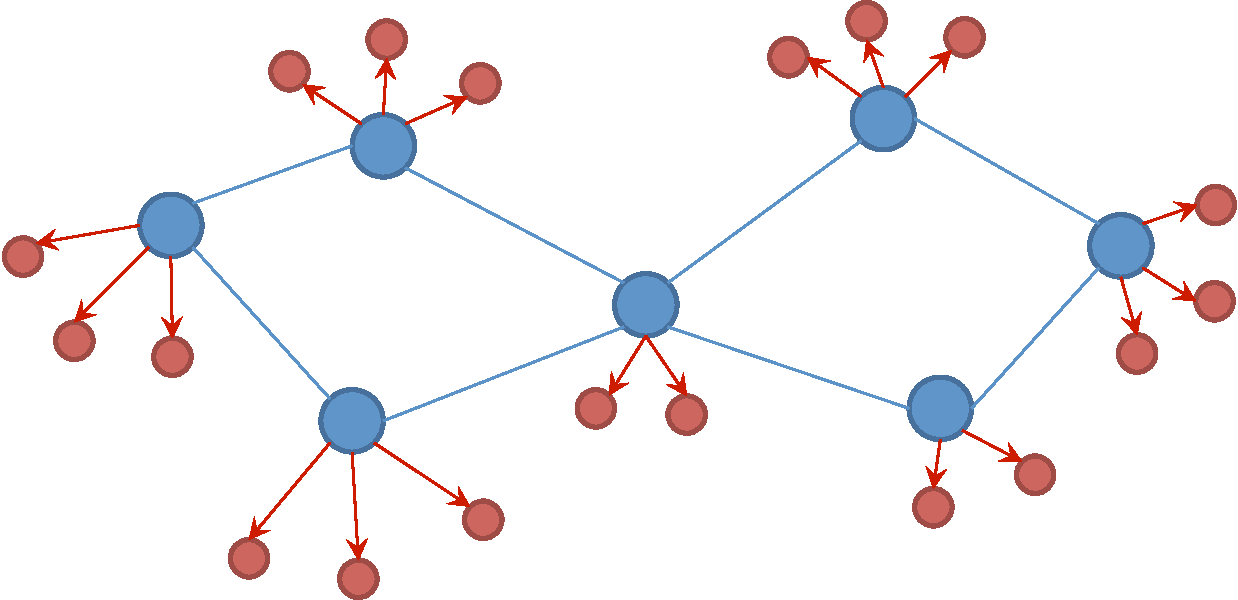
\includegraphics[width=0.8\textwidth]{pt_show.pdf}
    \caption{This figure shows the two-level formulation of the
      proposed optimization formulation. At the first level, each
      center image (depicted by blue circles) are connected to all its
    neighbors (red circles) within the same cluster, and at the second level,
    different centers are connected via parallel transport
    contraints. }
    \label{fig:pt_show}
\end{figure}


Given a set of $n$ images, we first group them into
$m$ clusters, using K-medoid, where each cluster has a \emph{center
  image}. The number of clusters $m$ is choosen via cross validation,
such that all samples within a cluster are close enough to the
corresponding center.
Suppose the $i$-th cluster contains $n_i$ samples. For this cluster, 
we use $I_{i,0}$ to denote the center image of this, and $I_{i,j}$
(with $j = 1, \ldots, n_i$) to the $j$-th non-center image. 
%
Here, we consider each center image as the representation of the canonical
shape of an object, and other images in the same cluster as generated
by deforming the center image.

As discussed in previous section, a deformation group can be
characterized by a Lie algebra. Therefore, the problem of learning the
deformation groups thus reduces to the one of estimating the Lie
algebraic basis for each cluster. Here, we denote the basis for the
$i$-th cluster by $\bset_i = (B_{i,1}, \ldots, B_{i,K})$.
To estimate these basis, we formulate an optimization problem, of
which the objective function comprises two levels of terms, as shown
in Figure~\ref{fig:pt_show}.


\subsubsection{Within-cluster Level.}
%
Applying the deformation group characterized by the Lie
algebraic basis $\bset_i$ to the image $I_{i,0}$ yields a
$K$-dimensional manifold comprised of all the deformed images,
denoted by $G(\bset_i) \circ I_{i,0}$, as
\begin{equation}
    G(\bset_i) \circ I_{i,0} \triangleq
    \{ \exp(V) \circ I_{i,0}: V \in \ga(\bset_i) \}.
\end{equation}
Here, $\ga(\bset_i)$ denotes the Lie algebraic space spanned by
$\bset_i$.
With the assumption that $I_{i,j}$ is generated by deforming
$I_{i,0}$, we expect that the $I_{i,j}$ is close to
$G(\bset_i) \circ I_{i,0}$. Particularly, the distance from $I_{i,j}$
to $G(\bset_i) \circ I_{i,0}$ is given by
\begin{equation}
    \dist(I_{i,j}, G(\bset_i) \circ I_{i,0})
    = \min_{\valpha} \left\| I_{i,j} -
      \exp \left(\sum_{k=1}^K \alpha^k B_{i,k} \right) \circ I_{i,0}
    \right\|.    
\end{equation}
When the deformed image $I_{i,j}$ is close to the center $I_{i,0}$,
the coefficients are small. Consequently, by
Eq.\eqref{eq:liealg_actiond}, we can approximately write
\begin{equation}
    \exp \left( \sum_{k=1}^K \alpha^k B_{i,k} \right) \circ I_{i,0}
    \simeq
    I_{i,0} + \sum_{k=1}^K \alpha^k (B_{i,k} \circ I_{i,0}).
\end{equation}
As a result, we have
\begin{align} \label{eq:approx_dist2}
    \dist(I_{i,j}, G(\bset_i) \circ I_{i,0})^2
    &\simeq
    \min_{\valpha} \left \|
      (I_{i,j} - I_{i,0}) -
      \sum_{k=1}^K \alpha^k (B_{i,k} \circ I_{i,0})
    \right \|^2 \notag \\
    &=
    \min_{\valpha} \sum_{\vx \in \dset} \left(
      (I_{i,j}(\vx) - I_{i,0}(\vx)) +
      \sum_{k=1}^K \alpha^k B_{i,k}(\vx)^T \nabla I_{i,0}(\vx)
    \right)^2.
\end{align}
Here, $\dset$ is the set of all observable pixel locations.
For convenience, we define
\begin{equation}
    Q_{ij}(\bset_i, \valpha_{i,j}) =
    \left \| (I_{i,j} - I_{i,0}) -
      \sum_{k=1}^K \alpha_{i,j}^k (B_{i,k}
      \circ I_{i,0})
    \right \|^2.
\end{equation}
Note that $Q_{ij}$ is a quadratic \wrt~$\valpha_{i,j}$. Hence, the
optimal coefficients that yield the minimum (approximate) distance can
be readily solved, given $\bset_i$.


\subsubsection{Inter-Cluster Level.}
%
The basis associated with different groups are related to each other
via parallel transport. Specifically, we establish a higher-level
network between cluster centers, where each center image is connected
to several \emph{neighboring centers}, \ie~other centers that are not
too far from it, such that the optical flow between them can be
reliably estimated.

For each pair of neighboring centers $I_{i,0}$ and $I_{i',0}$, we
estimate the dense correspondence between them $T_{ii'}$ and
$T_{i'i}$, using an optical flow algorithm~\cite{OF}.
Ideally, we would expect the basis $\bset_{i}$ to be the transported
version of $\bset_{i'}$ \wrt~the transform $T_{i'i} = T_{ii'}^{-1}$,
\ie~$B_{i,k} = T_{ii'}^{-1} \tsp B_{i',k}$, and vice versa. As some errors
may be incurred in optical flow estimation, we use the quadratic term as
follows to penalize the deviation from this relation:
\begin{equation}
    H_{ii'}(\bset_i, \bset_{i'}) = \sum_{k=1}^K \|B_{ik} - T_{ii'}^{-1} \tsp B_{i',k} \|^2
\end{equation}
Here, we have
\begin{equation}
    \| B_{ik} - T_{ii'}^{-1} \tsp B_{i,k} \|^2
    = \sum_{\vx \in \dset \cap T_{ii'}(\dset)}
    \| B_{ik}(\vx) -
    \mJ_{T_{ii'}}(T_{ii'}(\vx)) B_{i'k}(T_{ii'}(\vx))
    \|.
\end{equation}
Here, $T_{ii'}(\vx)$ is the location of the pixel on $I_{i',0}$
that corresponds to the pixel at $\vx$ of $I_{i,0}$.
In general, $T_{ii'}(\vx)$ does not yield integer coordinates.
Under such circumstances, linear interpolation can be used to
derive the values of $\mJ_{T_{ii'}}(T_{ii'}(\vx))$ and
$B_{ik}(T_{ii'}(\vx))$.
In addition, $\vx \notin T_{ii'}(\dset)$ indicates that the pixel at
$\vx$ of $I_{i,0}$ is transformed outside of the observable region,
and thus the corresponding term is not included. 



\subsubsection{Joint Formulation.}
%
Integrating the terms at both levels, we derive the joint objective
function as follows. 
\begin{equation}
    L(\bset) =
    \sum_{i=1}^m \sum_{j=1}^{n_i} \min_{\valpha} Q_{ij}(\bset_i,
    \valpha)
    +
    \gamma \sum_{i=1}^m \sum_{i' \in \nset_i} H_{ii'}(\bset_i, \bset_i').
\end{equation}
Here, $\nset_i$ is a set consisting of the indices of $I_{i,0}$'s
neighboring centers, and $\gamma$ is a positive weight that controls
the contribution of the parallel transport constraints.
To minimize this function, we introduce an
auxiliary function that involves $\valpha_{i,j}$ as arguments:
\begin{equation}
    L_{aux}(\bset, \valpha) =
    \sum_{i=1}^m \sum_{j=1}^{n_i} Q_{ij}(\bset_i,
    \valpha_{i,j})
    +
    \gamma \sum_{i=1}^m \sum_{i' \in \nset_i} H_{ii'}(\bset_i, \bset_i').
\end{equation}
Obviously, $L_{aux}$ gives an upper bound of $L$ and has
\begin{equation}
    L(\bset) = \min_{\alpha} L_{aux}(\bset, \valpha).
\end{equation}
Consequently, $L(\bset)$ can be optimized by alternating the updates of
$\valpha$ and $\bset$:
\begin{align}
    \hat{\valpha}_{i,j}^{(t)}
    &\leftarrow \argmin_{\valpha} \ Q_{ij}(\bset_i^{(t-1)}, \valpha),
    \\
    \hat{\bset}_i^{(t)}
    &\leftarrow \argmin_{\bset} \
    \sum_{j=1}^{n_i} Q_{ij}(\bset, \valpha_{i,j}^{(t)}) +
    \gamma \sum_{i' \in \nset_i} H_{ii'}(\bset_i, \bset_{i'}).
\end{align}
Note that the value of $L_{aux}(\bset, \valpha)$ decreases with each
updating step. Particularly, the values of $L$ and $L_{aux}$ become
equal each time when $\valpha$ is updated to the optima,
\ie~$L(\bset^{(t)}) = L_{aux}(\bset^{(t)}, \valpha^{(t+1)})$. 


\subsection{Initialization}

While $L_{aux}$ is convex \wrt~$\bset$ and $\valpha$ respectively,
this is not a convex optimization problem jointly. Hence, appropriate
initialization is crucial as to obtaining a reasonably good solution.
Here, we describe a simple yet effective scheme to initialize the
the basis $\bset$.

We choose a particular cluster as the ``standard cluster'', and
compute the optical flow~\cite{OF} from the center of this standard cluster to
the centers of other clusters. With these optical flows, we can warp
the images in other clusters towards the standard one. For example,
suppose $I_{1,0}$ is selected as the standard, and the optical flow
from $I_{1,0}$ to $I_{2,0}$ is $T_{12}$, then we warp each image in
the second cluster as $I'_{2,j} = T_{12}^{-1}(I_{2,j})$ for $j = 0, 1,
\ldots, n_2$.
In this way, for each non-standard cluster, we acquire a warped center
as well as a set of warped images, which are considered as
generated by deforming the warped center.

At the initialization stage, we assume that the standard cluster and
the warped clusters share the same basis. To estimate this basis, we
compute the optical flow fields from the standard center to other
images in the standard cluster, and those from each warped center to
other images in the corresponding cluster. All these flow fields can
be roughly considered as residing near the space spanned by the shared
basis. Therefore, the basis can be estimated by applying principal
component analysis (PCA) to these optical flow fields pooled
together.
%
After the basis associated with the standard cluster have been
initialized as above, the basis for other clusters can be readily
obtained via parallel transport. 











%%% Local Variables:
%%% TeX-master: "main_paper"
%%% End:
